\section{Cryptography}\label{sec:5-cryptography}

In modern cryptography, security is often based on practical computational constraints. A key example is \textbf{RSA encryption}, which relies on the difficulty of factoring large integers and is widely used in internet security. In RSA, the sender and receiver generate a \textbf{public key} and a \textbf{private key} respectively: the public key is shared openly and used to encrypt the message, while the private key is kept secret and used to decrypt it.

\subsection{Classical key distribution}\label{subsec:5-classical-key-distribution}
Let us consider two users, Alice and Bob, who want to communicate securely in the presence of a third party, Eve, who tries to read the message.

Bob performs the following steps:
\begin{itemize}
    \item Choose two large prime numbers, $p$ and $q$;
    \item Compute $n = p q$ and publish it on the public channel;
    \item Compute $\varphi(n) = (p-1)(q-1)$;
    \item Choose an integer $e$ such that $\gcd(e,\varphi(n))=1$, and publish it on the public channel;
    \item Compute the private exponent $d$ as the modular inverse of $e$ modulo $\varphi(n)$, namely
    \[
    d \equiv e^{-1} \pmod{\varphi(n)}.
    \]
\end{itemize}
Here $\gcd$ denotes the greatest common divisor, i.e. the largest positive integer dividing both numbers. The notation $x \equiv y \pmod{n}$ means that $x-y$ is an integer multiple of $n$.

Alice then does the following:
\begin{itemize}
    \item Choose the message $M$;
    \item Compute the encrypted message
    \[
    C \equiv M^e \pmod{n};
    \]
    \item Send $C$ to Bob through the public channel.
\end{itemize}
Bob decrypts the message by computing
\[
M \equiv C^d \pmod{n}.
\]
The security of RSA relies on the fact that Eve knows $n$ and $e$, but in order to find $d$ she would need to factorize $n$ into $p$ and $q$. For \textbf{sufficiently large} $n$ this is \textbf{computationally infeasible} with classical algorithms. However, quantum computers would be able to solve the factoring problem efficiently using Shor's algorithm.

\subsection{Quantum key distribution}\label{subsec:quantum-key-distribution}
Suppose that a beam of light is sent onto a \textbf{polarized beam splitter}. Three cases are relevant:
\begin{itemize}
    \item \textbf{State} $\ket{H}$: the light is horizontally polarized and is transmitted to detector $D_1$.
    \item \textbf{State} $\ket{V}$: the light is vertically polarized and is reflected to detector $D_2$.
    \item \textbf{State} $\ket{\theta}$: the light is prepared in a superposition of horizontal and vertical polarization, so both detectors may receive a signal with different probabilities.
\end{itemize}
\begin{figure}[H]
    \centering
    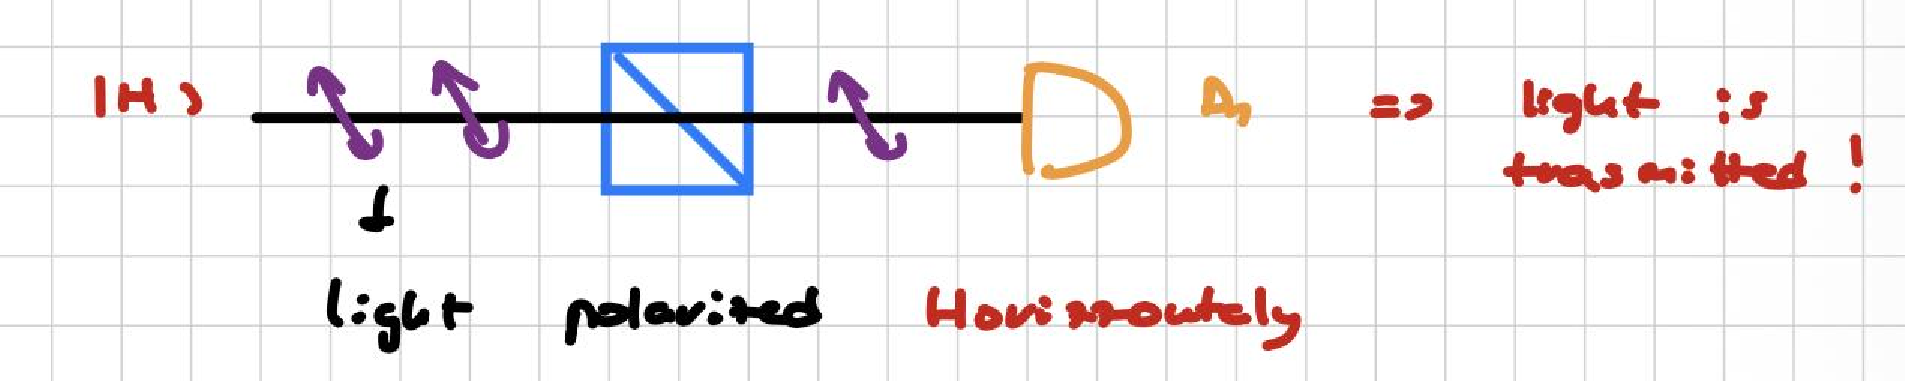
\includegraphics[width=0.9\linewidth]{images_in_pdf/5-/Grafico_21.pdf}
\end{figure}
\begin{figure}[H]
    \centering
    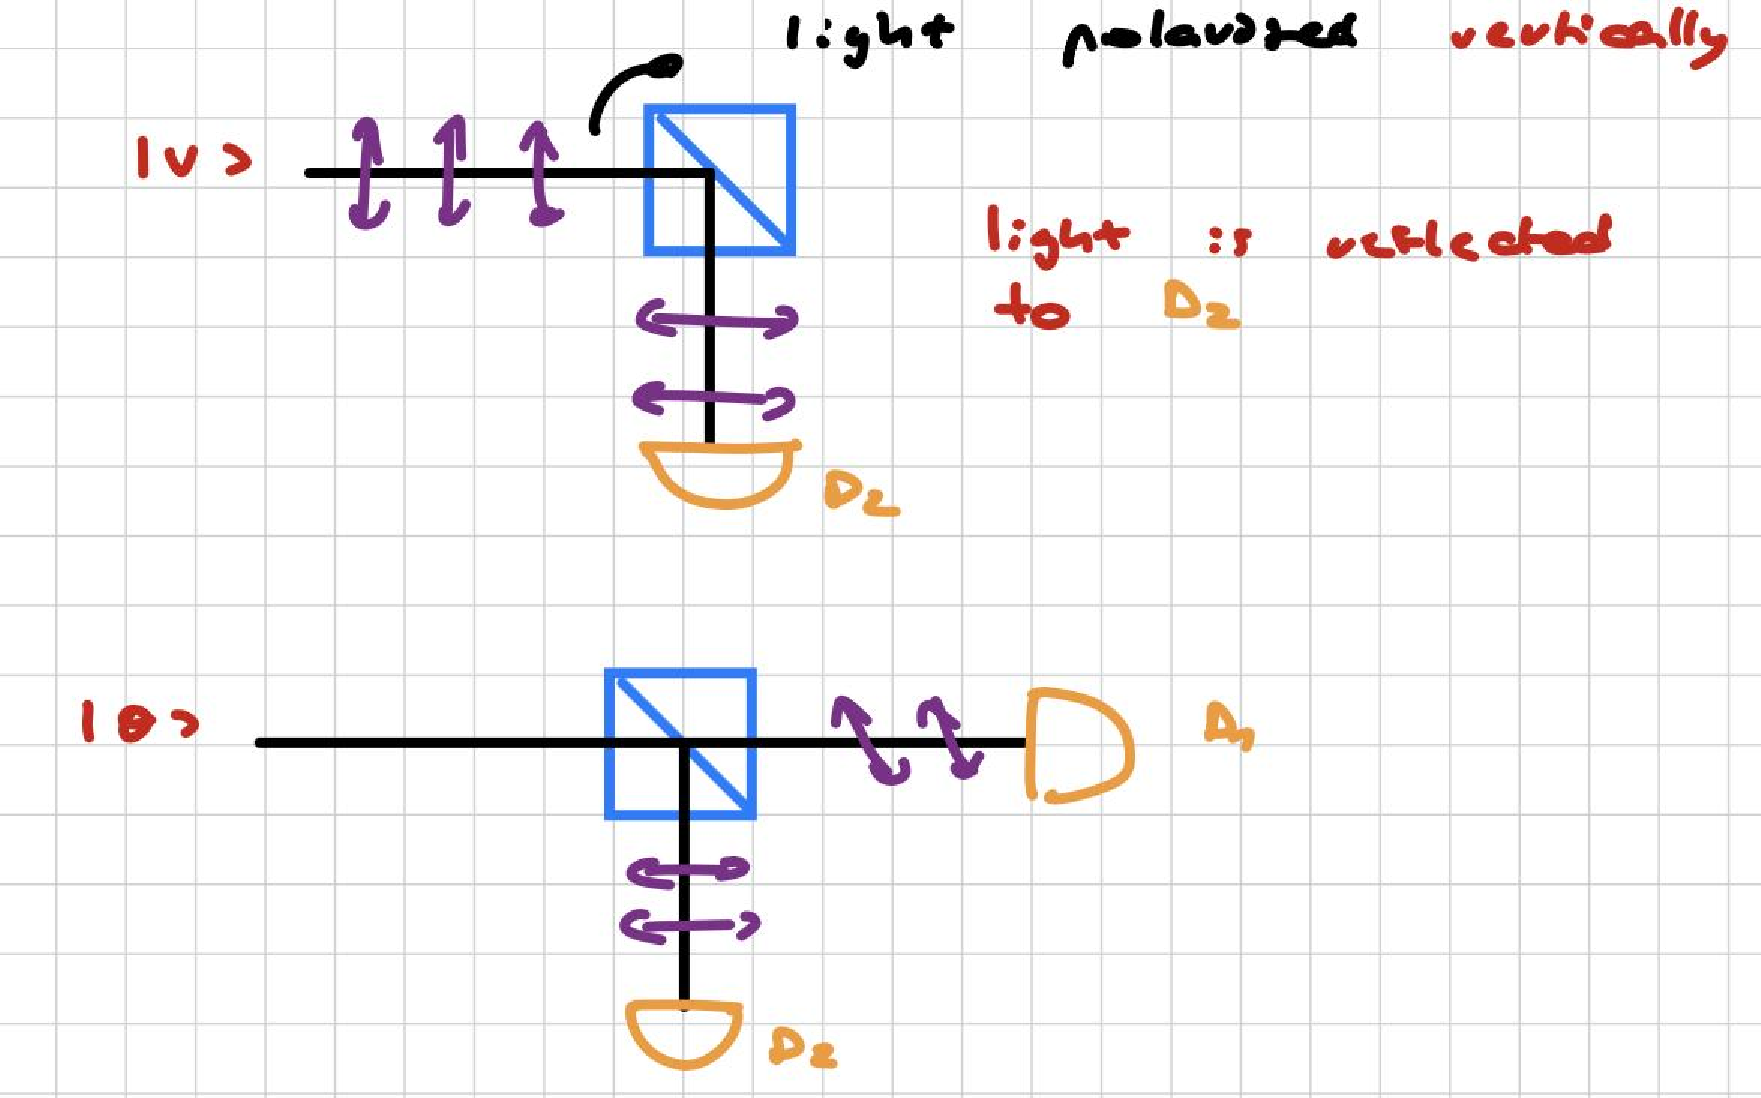
\includegraphics[width=0.8\linewidth]{images_in_pdf/5-/Grafico_22.pdf}
\end{figure}

For a generic linearly polarized state,
\[
\ket{\theta} = \cos(\theta)\ket{H} + \sin(\theta)\ket{V},
\]
the probabilities of obtaining the two outcomes are
\[
P_H = |\braket{H|\theta}|^2 = \cos^2(\theta),
\qquad
P_V = |\braket{V|\theta}|^2 = \sin^2(\theta).
\]
For a diagonal state, we define
\[
\ket{D_+} = \frac{1}{\sqrt{2}}\left(\ket{H}+\ket{V}\right),
\qquad
\ket{D_-} = \frac{1}{\sqrt{2}}\left(\ket{H}-\ket{V}\right).
\]
These states are orthogonal and form another basis of the polarization Hilbert space. In this way, polarized photons can be used to encode one bit of information.

The key idea is that Alice and Bob want to communicate, while Eve wants to intercept the message. If Eve measures a photon in the same basis used by Alice, she can reproduce the state correctly. However, if she measures in the wrong basis, the state is disturbed. When she re--sends the photon to Bob, her intervention becomes detectable. Thus, \hl{the measurement process modifies the quantum state itself}, revealing Eve's presence.

\question{Why not make copies of the original state and measure the copies instead?}{This is impossible because of the \textbf{no-cloning theorem}.}

\textbf{Proof idea:} suppose a ``quantum Xerox machine'' exists, i.e. a device that takes an unknown state $\ket{\psi}$ and a blank state $\ket{X}$ and produces two identical copies:
\[
\ket{\psi}\ket{X} \longrightarrow \ket{\psi}\ket{\psi}.
\]
Assume that the machine works for the basis states $\ket{H}$ and $\ket{V}$:
\[
\ket{H}\ket{X} \longrightarrow \ket{H}\ket{H},
\qquad
\ket{V}\ket{X} \longrightarrow \ket{V}\ket{V}.
\]
Because quantum evolution is linear, it should also work for the superposition
\[
\ket{D_+} = \frac{1}{\sqrt{2}}\left(\ket{H}+\ket{V}\right).
\]
Linearity would imply
\[
\ket{D_+}\ket{X} \longrightarrow \frac{1}{\sqrt{2}}\left(\ket{H}\ket{H}+\ket{V}\ket{V}\right),
\]
whereas perfect cloning would require
\[
\ket{D_+}\ket{X} \longrightarrow \ket{D_+}\ket{D_+}
= \frac{1}{2}\left(\ket{H}\ket{H}+\ket{H}\ket{V}+\ket{V}\ket{H}+\ket{V}\ket{V}\right).
\]
These two results are different, so a universal cloning machine cannot exist.

\callout{No cloning theorem - Alternative proof}{%
\begin{proof}
Suppose there exists a unitary operator $U=U^\dagger$ such that:
\begin{equation*}
\begin{cases}
    U\ket{\psi}\otimes\ket{\phi} = \ket{\psi}\otimes\ket{\psi}\\
    U\ket{\varphi}\otimes\ket{\phi} = \ket{\varphi}\otimes\ket{\psi}
\end{cases}
,\quad \forall \ket{\psi}, \ket{\varphi}, \ket{\phi} \in \mathcal{H},
\end{equation*}
where the states are normalized. Since unitary operators preserve inner products, it should hold that:
\begin{equation*}
    \left(\bra{\psi}\otimes\bra{\phi}\right)
    \left(\ket{\varphi}\otimes\ket{\phi}\right) =
    \left(\bra{\psi}\otimes\bra{\psi}\right)
    \left(\ket{\varphi}\otimes\ket{\varphi}\right)
\end{equation*}

following $\braket{\phi|\phi} = 1$:
\begin{equation*}
    \braket{\psi|\varphi} = \braket{\psi|\varphi}\braket{\psi|\varphi}
\end{equation*}

and this is only possible if the inner product $\braket{\psi|\varphi}$ is either $0$ or $1$. In other words, the states $\ket{\psi}$ and $\ket{\varphi}$ must be either \textbf{orthogonal} or \textbf{identical} up to a phase, which contradicts the assumption that the cloning operator works for all states.
\end{proof}
}

For this reason, Alice can send Bob a string of bits encoded in single photons prepared in one of the polarization states $\ket{H}$, $\ket{V}$, $\ket{D_+}$, or $\ket{D_-}$, while choosing the basis at random. Eve cannot copy the photons without introducing errors. By comparing a subset of their bits, Alice and Bob can detect whether the channel has been intercepted.

\subsection{BB84: first Quantum Cryptography Protocol}\label{subsec:BB84}
The BB84 protocol is a quantum key distribution scheme. It does not directly encrypt the message; rather, it allows Alice and Bob to \hl{generate a shared secret key}, which can later be used in a one-time pad.

The encrypted message is obtained by adding, modulo $2$, the message bits and a secret random key of the same length. For example,
\[
0 \oplus 0 = 0,\qquad 1 \oplus 0 = 1,\qquad 0 \oplus 1 = 1,\qquad 1 \oplus 1 = 0.
\]
Bob can decrypt the message using the same key.

The two bases used in BB84 are:
\begin{itemize}
    \item \textbf{Rectilinear basis} $+$: $\ket{H} \mapsto 0$ and $\ket{V} \mapsto 1$;
    \item \textbf{Diagonal basis} $\times$: $\ket{D_+} \mapsto 0$ and $\ket{D_-} \mapsto 1$.
\end{itemize}
The experimental setup consists of:
\begin{itemize}
    \item[--] a single-photon source;
    \item[--] polarization preparation optics, such as polarizers and wave plates;
    \item[--] a polarizing beam splitter, which separates the two orthogonal polarizations into transmitted and reflected outputs;
    \item[--] two single-photon detectors.
\end{itemize}
The protocol proceeds as follows:
\begin{enumerate}
    \item Alice randomly chooses a basis and a bit value, then sends the corresponding photon state.
    \item Bob randomly chooses a measurement basis and records the detector outcome.
    \item After the transmission, Alice and Bob publicly compare their basis choices and keep only the events where the bases match. 
\end{enumerate}
The possible configurations are summarized in Table~\ref{tab:bb84}.

\begin{table}[H]
\label{tab:bb84}
\centering
\renewcommand{\arraystretch}{1.3}
\begin{tabular}{|c|c|c||c|c|c||c|}
\hline
\multicolumn{3}{|c||}{\textbf{Alice (A)}} & 
\multicolumn{3}{c||}{\textbf{Bob (B)}} & 
\textbf{Basis} \\
\textbf{Basis} & \textbf{State} & \textbf{Bit} &
\textbf{Basis} & $D_1$ & $D_2$ &
\textbf{Match} \\
\hline
$+$ & $\ket{H}$ & 0 & $+$ & 100\% & 0\% & Yes \\
$+$ & $\ket{V}$ & 1 & $+$ & 0\% & 100\% & Yes \\
$\times$ & $\ket{D_+}$ & 0 & $+$ & 50\% & 50\% & No \\
$\times$ & $\ket{D_-}$ & 1 & $+$ & 50\% & 50\% & No \\
$+$ & $\ket{H}$ & 0 & $\times$ & 50\% & 50\% & No \\
$+$ & $\ket{V}$ & 1 & $\times$ & 50\% & 50\% & No \\
$\times$ & $\ket{D_+}$ & 0 & $\times$ & 100\% & 0\% & Yes \\
$\times$ & $\ket{D_-}$ & 1 & $\times$ & 0\% & 100\% & Yes \\
\hline
\end{tabular}
\caption{BB84 quantum key distribution protocol: polarization states, measurement bases, and basis matching.}
\end{table}


The measurement operators associated with the two bases can be written as
\begin{equation}\label{5-measurement-operators}
\hat{M}_{+} = \ket{H}\bra{H} - \ket{V}\bra{V},
\qquad
\hat{M}_{\times} = \ket{D_+}\bra{D_+} - \ket{D_-}\bra{D_-}.
\end{equation}

So that, for example, the action of $\hat{M}_+$ on the $+$ and $\times$ basis states is:
\begin{equation}\label{5-measurement-operators-action}
\begin{cases}
\hat{M_+} \ket{H} = 1 \cdot \ket{H}\\
\hat{M_+} \ket{V} = -1 \cdot \ket{V}
\end{cases}
\hspace{1cm}
\begin{cases}
\hat{M_+} \ket{D_+} = 
\tfrac{1}{\sqrt{2}} \left(\ket{H} -\ket{V}\right) \equiv \ket{D_-}\\ 
\hat{M_+} \ket{D_-} = 
\tfrac{1}{\sqrt{2}} \left(\ket{H} +\ket{V}\right) \equiv \ket{D_+}
\end{cases}
\end{equation}

While $\ket{H}$ and $\ket{V}$ are its eigenstates with eigenvalues $1$ and $-1$ respectively, when it acts on $\ket{D_{\pm}}$ a superposition of the states $\ket{H}$ and $\ket{V}$ is returned.

\calloutinfo{If Alice and Bob choose the same basis, the bit value is preserved. If they choose different bases, the measurement outcome is random.}

\question{What happens if Eve intercepts the photon?}{
Suppose Alice uses the $+$ basis:
\begin{itemize}
    \item if Eve and Bob both choose the $+$ basis, Eve reads the right bit and re--sends the correct photon and Bob reads the correct bit;
    \item if Eve chooses the $+$ basis but Bob chooses the $\times$ basis, Bob obtains a random result, the bit would be discarded anyway;
    \item if Eve chooses the $\times$ basis and Bob chooses the $+$ basis, Bob again obtains a random result;
    \item if Eve and Bob both choose the $\times$ basis, Eve has already disturbed the state and Bob may obtain the wrong result after basis reconciliation.
\end{itemize}
The same reasoning applies if Alice initially chooses the $\times$ basis.
}

Alice and Bob do not keep all transmitted bits. Instead, they generate a longer raw key, publicly compare a subset of the bits, and discard the mismatched ones. For example, if they need a final key of 1064 bits, they may transmit a longer string, reveal a sample of check bits, and keep the rest.

If Alice reveals the first bit as $(+,0)$ then an intercept--resend attack by Eve has the following structure:
\begin{equation}\label{5-eve-attack}
A(+,0) \implies
\begin{cases}
E[P=50\%, +,0] \implies B[P=100\%, +,0] \implies P_{\text{tot}} = 50\% \\
E[P=50\%, \times, (0,1)] \implies
\begin{cases}
B[P=50\%, +,0] \implies P_{\text{tot}} = 25\% \\
B[P=50\%, +,1] \implies P_{\text{tot}} = 25\%
\end{cases}
\end{cases}
\end{equation}

\hl{In $3/4$ of the cases, Eve can get away with the single--bit attack}, which means that the detection probability is
\[
P_{\text{detected}} = 25\%,
\qquad
P_{\text{undetected}} = 75\%.
\]
If Eve attacks $n$ independent bits, the probability of remaining undetected is
\[
P_{\text{undetected}} = \left(\frac{3}{4}\right)^n,
\]
so the \textbf{probability of detecting} Eve is
\[
P_{\text{detected}} = 1 - \left(\frac{3}{4}\right)^n.
\]
For sufficiently large $n$, this probability becomes very close to $1$.

Eve's not the only source of error, others are:
\begin{itemize}
    \item photon loss during transmission;
    \item inefficient coupling to the detector;
    \item detector inefficiency;
    \item birefringent materials, which may rotate or distort the polarization during propagation;
    \item detector noise.
\end{itemize}

All these will increase the number of discarded bits and a overall reduction of the data transfer rate. We need to apply \textbf{error correction} by a parity check on a subset of bits;

\question{Which is the right number of bits?}{%
This is given by \textbf{Shannon's Noisy Channel Coding Theorem:} 
\begin{equation}\label{5-shannon}
N_{needed} = N \cdot [-\epsilon\cdot log_2(\epsilon)-(1-\epsilon)\cdot log_2(1-\epsilon)]
\end{equation}
where $N =$ total number of bits and $\epsilon = $ error propagation, if 
\[\epsilon \to + \infty \implies N_{needed} \to +\infty\] 
which means that we need to make sure that:
\begin{equation}\label{5-shanon-condition}
    \epsilon << \epsilon_{Eve}
\end{equation}
}

We also need an \textbf{authentication process} which consists in an exchange of few bits between Alice and Bob at the beginning according to a key, in this way Alice is sure to be communicating with Bob.